\documentclass[11pt]{article}

\usepackage[margin=1in]{geometry}
\usepackage{amsmath,amssymb}
\usepackage{graphicx}
\usepackage[numbers,sort]{natbib}
\usepackage[hidelinks]{hyperref}
\usepackage{booktabs}
\usepackage{array}
\usepackage{tabularx}
\usepackage{longtable}
\usepackage{caption}
\usepackage{xcolor}

\newcolumntype{L}[1]{>{\raggedright\arraybackslash}p{#1}}
\newcolumntype{Y}{>{\raggedright\arraybackslash}X}

% numbers regenerated from analysis/ by scripts/dataset_report_assets.py
\newcommand{\probeAll}{0.974}
\newcommand{\probeSize}{0.961}
\newcommand{\probeIntensity}{0.710}
\newcommand{\ispyRepeated}{941}
\newcommand{\ispyCases}{982}
\newcommand{\ispyPhasesMin}{4}
\newcommand{\ispyPhasesMax}{11}
\newcommand{\ispyComponents}{150}
\newcommand{\breadmFloatCases}{147}
\newcommand{\breadmCases}{232}
\newcommand{\busiBlocky}{97}
\newcommand{\busiPaperDoppler}{97}
\newcommand{\busiPaperMarker}{94}
\newcommand{\totalImages}{67,579}
\newcommand{\totalUsed}{53,166}
\newcommand{\breadmTestUnused}{446}
\newcommand{\cmmdUnlabeled}{1,456}
\newcommand{\cesmMissing}{5}
\newcommand{\mgCrossCandidates}{4.1 million}
\newcommand{\buscotOverlap}{2,655}
\newcommand{\buscotUsable}{3,599}
\newcommand{\buscotUsablePatients}{1,050}
\newcommand{\buscotRelabelled}{8}
\newcommand{\odeliaCentreAcc}{93}
\newcommand{\odeliaCentreChance}{34}
\newcommand{\odeliaCentreOnlyAUC}{0.71}
\newcommand{\odeliaStatsAUC}{0.76}
\newcommand{\cbisCrossSplitPatients}{16}
\newcommand{\cbisCrossSplitCrops}{57}
\newcommand{\cbisBWC}{379}
\newcommand{\cbisFull}{187}
\newcommand{\cbisFullLabels}{113}

\makeatletter\newcommand{\tableinput}[1]{\@@input #1 }\makeatother

\title{Sixteen Public Breast-Imaging Datasets:\\Provenance, Label Confirmation, and an Image-Level Audit}
\author{Nouran Fadlallah}
\date{October 2026}

\begin{document}
\maketitle

\begin{abstract}
This report audits the sixteen public breast-imaging datasets used or
considered in the multi-modal fusion project: six ultrasound sets (BUS-BRA,
BUSI, BUSC, BrEaST, BUS-CoT, BUS-UCLM), six mammography and tomosynthesis sets
(mini-MIAS, CDD-CESM, CMMD, BCS-DBT, CBIS-DDSM, DMID) and four DCE-MRI sets
(BreastDM, ISPY2 from BreastDCEDL, ODELIA, AMBL). For each dataset it records the source,
citation count, typical use and acquisition, and whether its benign/malignant
labels were confirmed by pathology. It then reports an audit run on the
original files: \totalImages{} images, of which \totalUsed{} are used for
training. The audit covers image-quality statistics, near-duplicate
detection checked against the actual training splits, burnt-in annotation
detection, lesion statistics, and MRI volume statistics. Labels in six of the
sixteen datasets are fully confirmed by biopsy or pathology. Three findings
change the reported results: near-duplicate images span the train/validation
split or the folds in BUSI and BUSC, and four BUSI pairs carry opposite labels.
CMMD contains identical images under different patient IDs, including one
benign/malignant conflict. In the combined MRI branch, the malignant-only ISPY2
slices can be distinguished from BreastDM malignant slices with an AUC of
\probeAll{} using crop size and intensity statistics alone. Of the newly added
datasets, BUS-CoT turns out to contain every BUSI and BUS-BRA image already
used here, and in ODELIA the acquiring centre is identifiable from simple image
statistics (\odeliaCentreAcc\% accuracy) while also predicting benign versus
malignant (AUC \odeliaCentreOnlyAUC), a centre shortcut. Preparing the data
for training added two further findings: a classical line-removal step
rewrites most of each speckled image, and a style-transfer model trained
towards BUS-BRA reproduces its burnt-in calipers and text, which confirms
these annotations as a learnable image property. Of the three most recent
datasets, AMBL's segmentations do not record which lesion is benign, and
the documented order puts a fifth of the masks in the wrong breast. DMID's
laterality alone predicts malignancy (AUC 0.61). BUS-UCLM files one patient
under two IDs. Section~\ref{sec:planned} lists the planned datasets that have
not been analysed yet.
\end{abstract}

\section{Introduction}

The project trains benign-vs-malignant classifiers on each dataset alone and on
all modalities combined through a late-fusion model. Two decisions depend on a
careful look at the data itself rather than at the models trained on it.
\begin{itemize}
  \item \textbf{Validity of the reported results.} Duplicated images across
  splits, labels that were never confirmed by pathology, and image properties
  that correlate with the label without being caused by the disease can all
  inflate test metrics~\citep{degrave2021shortcuts}.
  \item \textbf{Storage.} To free disk space, the raw downloads (about 180\,GB)
  will be replaced by the much smaller preprocessed copies that training reads.
  Some properties exist only in the raw data: DICOM headers, native bit depth,
  full frames outside the training crops, and excluded samples. They have to
  be measured before deletion.
\end{itemize}

The audit extends the dataset-verification method of
\citet{siddique2026audit}, developed for breast ultrasound, to mammography,
tomosynthesis and DCE-MRI. That method covers intensity, contrast, sharpness
and entropy statistics; perceptual-hash and SSIM duplicate detection; z-score
outliers; and Doppler and measurement-marker detection.
Section~\ref{sec:datasets} describes each dataset, Section~\ref{sec:method}
the audit, Section~\ref{sec:results} the results, and
Section~\ref{sec:recommendations} the resulting recommendations.

\section{Datasets}
\label{sec:datasets}

Table~\ref{tab:provenance} summarizes the sixteen datasets. Citation counts are
for the paper that introduced each dataset, retrieved from Semantic Scholar on
7~October 2026. They indicate how widely each dataset is used, not its quality.
For pathology confirmation, a dataset is marked \emph{Yes} only when its own
paper states that the labels come from biopsy or pathology reports;
\emph{Partial} when some labels instead come from imaging follow-up;
and \emph{Not stated} when the labels come from radiologists' reading.

\begin{table}[!htbp]
  \centering
  \footnotesize
  \setlength{\tabcolsep}{4pt}
  \caption{Provenance and label confirmation. Citations: Semantic Scholar, 7~Oct 2026, for the dataset paper.}
  \label{tab:provenance}
  \begin{tabularx}{\textwidth}{@{}l l Y r L{2.0cm} L{2.6cm}@{}}
    \toprule
    Dataset & Mod. & Source / host & Citations & License & Pathology-confirmed \\
    \midrule
    BUS-BRA~\citep{gomezflores2024busbra} & US & INCA, Rio de Janeiro; Zenodo & 193 & CC BY 4.0 & Yes (biopsy) \\
    BUS-CoT~\citep{yu2025buscot} & US & Aggregate of public sources; Figshare & 7 & CC BY 4.0 & Inherited per source$^{e}$ \\
    BUSI~\citep{aldhabyani2020busi} & US & Baheya Hospital, Cairo & 2,476 & not stated & Not stated \\
    BUS-UCLM~\citep{busuclm2025mendeley} & US & Univ.\ of Castilla-La Mancha; Mendeley Data & --$^{g}$ & CC BY 4.0 & Not stated \\
    BUSC~\citep{busc2023mendeley} & US & Mendeley Data (from \citep{rodrigues2017bus}) & 82$^{a}$ & not stated & Not stated \\
    BrEaST~\citep{pawlowska2024breast} & US & Polish medical centres; TCIA & 137 & CC BY 4.0 & Partial (biopsy or follow-up) \\
    mini-MIAS~\citep{suckling1994mias} & MG & UK screening films; PEIPA/Cambridge & 1,528$^{b}$ & CC BY & Not stated \\
    CDD-CESM~\citep{khaled2022cddcesm} & MG & NCI, Cairo University; TCIA & 73 & CC BY 4.0 & Partial (pathology or follow-up) \\
    CMMD~\citep{cai2023cmmd} & MG & SYSUCC \& Nanhai Hospital; TCIA & 69 & CC BY 4.0 & Yes (core-needle biopsy) \\
    BCS-DBT~\citep{buda2021bcsdbt} & DBT & Duke Health; TCIA & 120 & CC BY-NC 4.0 & Yes for Benign/Cancer$^{c}$ \\
    CBIS-DDSM~\citep{lee2017cbisddsm} & MG & DDSM film archive (US); TCIA & 873 & CC BY 3.0 & Yes, except ``without callback''$^{f}$ \\
    DMID~\citep{oza2024dmid} & MG & India (DA-IICT); Figshare & --$^{g}$ & CC BY 4.0 & Not stated \\
    BreastDM~\citep{zhao2023breastdm} & MRI & Taizhou Central Hospital; GitHub & 75 & not stated & Yes (histology) \\
    ISPY2~\citep{fridman2026breastdcedl} & MRI & I-SPY2 trial sites; TCIA (BreastDCEDL) & 8$^{d}$ & CC BY-NC-ND 4.0 & Yes (trial entry) \\
    ODELIA~\citep{mullerfranzes2025odelia} & MRI & Six European centres; Hugging Face & 6 & CC BY-NC 4.0 & Partial (histopathology or 2-year follow-up) \\
    AMBL~\citep{daniels2024ambl} & MRI & Single centre (1.5\,T GE); TCIA & --$^{g}$ & CC BY 4.0 & Partial (biopsy/surgery or 1-year follow-up) \\
    \bottomrule
  \end{tabularx}
  \par\smallskip\footnotesize
  $^{a}$PDF-UNet~\citep{iqbalsharif2023pdfunet}, the paper associated with the BUSC release; the Mendeley dataset itself has no citable paper.
  $^{b}$1994 paper; the 2015 v1.21 data release~\citep{suckling2015miasv121} has a further 205.
  $^{c}$Normal and Actionable views are not biopsied.
  $^{d}$BreastDCEDL \emph{Scientific Data} paper (2026); the ISPY2 subset was first described in an arXiv preprint~\citep{fridman2025breastdcedl}.
  $^{e}$Labels come from each source dataset or, for web and article figures, from the accompanying text.
  $^{f}$BENIGN\_WITHOUT\_CALLBACK findings were judged benign without biopsy.
  $^{g}$Added 19--22 October 2026; citation counts not retrieved.
\end{table}

\subsection{Ultrasound}

\paragraph{BUS-BRA~\citep{gomezflores2024busbra}.}
\emph{Source:} National Institute of Cancer (INCA), Rio de Janeiro, Brazil;
distributed on Zenodo under CC~BY~4.0. \emph{Collection:} 1,875 anonymized
B-mode images of 1,064 women, typically two orthogonal views per lesion,
acquired during routine studies with four scanners (in this copy: GE Logiq~7,
902 images; GE Logiq~5, 809; Toshiba Aplio~300, 139; U-Systems, 25). A senior
ultrasonographer assigned BI-RADS 2--5 and outlined each lesion by hand.
\emph{Ground truth:} ``biopsy-proven tumors'' (722 benign and 342 malignant
cases) --- \textbf{pathology-confirmed}. \emph{Usage:} classification and
segmentation benchmarks. Its main advantage is the official case-level 5- and
10-fold partitions, which make results comparable across papers.

\paragraph{BUSI~\citep{aldhabyani2020busi}.}
\emph{Source:} Baheya Hospital for Early Detection \& Treatment of Women's
Cancer, Cairo, Egypt. \emph{Collection:} images of 600 women aged 25--75,
collected in 2018 on GE LOGIQ~E9 and E9~Agile scanners, stored as DICOM and
released as cropped PNGs (780 images, about 500$\times$500 pixels) with
lesion masks. \emph{Ground truth:} radiologists at Baheya reviewed and
corrected the annotations; the paper does not mention biopsy or pathology,
so labels are \textbf{not stated to be pathology-confirmed}. The paper's own
table lists 487 benign images, but its totals (780) match the 437 benign
images in the release. \emph{Usage:} the most widely used public breast
ultrasound set (2,476 citations), for classification, segmentation and
detection.

\paragraph{BUSC~\citep{busc2023mendeley}.}
\emph{Source:} Mendeley Data (2023), released with the PDF-UNet
work~\citep{iqbalsharif2023pdfunet}; the images are taken from an earlier
Mendeley ultrasound collection~\citep{rodrigues2017bus}. \emph{Collection:}
100 benign and 150 malignant BMP images with no masks and no patient
identifiers. The release page describes 64$\times$64 originals resized to
128$\times$128, but the local images have a median size of 93$\times$139
pixels and 46 distinct sizes. \emph{Ground truth:} annotated ``with the help
of an experienced radiologist'' --- \textbf{not pathology-confirmed} as far
as the release states. \emph{Usage:} small classification and semi-supervised
segmentation benchmark.

\paragraph{BrEaST-Lesions-USG~\citep{pawlowska2024breast}.}
\emph{Source:} medical centres in Poland, 2019--2022, five radiologists;
distributed on TCIA under CC~BY~4.0. \emph{Collection:} 256 scans from 256
patients with freehand tumour masks, the full BI-RADS descriptor set, patient
age, tissue composition and a histopathological diagnosis where available
(33 subtypes). \emph{Ground truth:} ``all tumors confirmed by follow-up care
or biopsy result''; some cases were confirmed by fine-needle aspiration
cytology --- \textbf{partially pathology-confirmed}. \emph{Usage:} a curated
benchmark; its paper also re-audits the older public ultrasound sets.

\paragraph{BUS-CoT~\citep{yu2025buscot}.}
\emph{Source:} Peking University and partner hospitals; Figshare, CC~BY~4.0.
\emph{Collection:} 11,439 images of 4,838 patients, gathered from
``open-access papers, publicly available case studies (like Radiopaedia and
PubMed), and open-access datasets''. It is therefore an aggregate of existing
public data: it contains all of BUSI and BUS-BRA, UDIAT Dataset~B, a teaching
library (TFUSL, likely \emph{The Free UltraSound Library}), Thammasat
University data (TUHD), and about 5,100 scraped web images and journal
figures. Six senior radiologists annotated image features, BI-RADS and
chain-of-thought reasoning. \emph{Ground truth:} histopathology categories were
``extracted from description texts'', so label quality is \textbf{inherited
from each source}. \emph{Usage:} vision--language reasoning and
rare-histology benchmarks.

\paragraph{BUS-UCLM~\citep{busuclm2025mendeley}.}
\emph{Source:} University of Castilla-La Mancha (Spain); Mendeley Data v3,
January 2025, CC~BY~4.0. \emph{Collection:} 683 B-mode images (856$\times$606)
of 38 patients from one scanner (Siemens ACUSON S2000), 2022--2023: 419
normal, 174 benign and 90 malignant, with RGB segmentation masks (green
benign, red malignant) and per-image flags for Doppler, caliper marks and
combined images. \emph{Ground truth:} how labels were confirmed is
\textbf{not stated}. \emph{Usage:} lesion segmentation.

\subsection{Mammography and tomosynthesis}

\paragraph{mini-MIAS~\citep{suckling1994mias}.}
\emph{Source:} Mammographic Image Analysis Society (UK); PEIPA and the
Cambridge repository~\citep{suckling2015miasv121}. \emph{Collection:} 322
digitized screen-film MLO mammograms (161 women, both breasts) from the UK
screening programme, reduced to 200\,$\mu$m pixels and padded to
1024$\times$1024. \emph{Ground truth:} a radiologist marked each abnormality
with a centre and radius and classified it as benign or malignant; no
pathology confirmation is described. \emph{Usage:} the classic CAD benchmark
(1,528 citations), now mostly used for small-scale classification and
segmentation experiments.

\paragraph{CDD-CESM~\citep{khaled2022cddcesm}.}
\emph{Source:} Radiology Department, National Cancer Institute, Cairo
University, January 2019 -- February 2021; TCIA, CC~BY~4.0.
\emph{Collection:} 2,006 images of 326 women aged 18--90: 1,003 low-energy
images and 1,003 recombined (subtracted) contrast-enhanced images, CC and MLO,
acquired on GE Senographe DS and Hologic Selenia Dimensions systems, with
BI-RADS reports and manual segmentations. \emph{Ground truth:} pathology is
the reference for suspicious lesions and imaging follow-up for benign-looking
ones --- \textbf{partially pathology-confirmed}. \emph{Usage:} CESM
classification and report-generation research.

\paragraph{CMMD~\citep{cai2023cmmd,cui2021cmmd}.}
\emph{Source:} Sun Yat-sen University Cancer Center (Guangzhou) and Nanhai
Affiliated Hospital of Southern Medical University (Foshan), July 2012 --
January 2016; TCIA, CC~BY~4.0. \emph{Collection:} 1,775 patients aged 18--87,
CC and MLO views on GE Senographe DS and Siemens Mammomat Inspiration systems.
Labels apply only to the affected breast. CMMD2 adds molecular subtypes for
749 patients. \emph{Ground truth:} ``biopsy samples were collected from all
patients by core needle biopsy'' --- \textbf{pathology-confirmed}.
\emph{Usage:} benign/malignant classification and molecular-subtype prediction
in a non-Western population.

\paragraph{BCS-DBT~\citep{buda2021bcsdbt}.}
\emph{Source:} Duke Health, August 2014 -- January 2018; TCIA, CC~BY-NC~4.0.
\emph{Collection:} 5,060 patients and 5,610 tomosynthesis studies. The local
copy is the validation release: 1,163 views of 280 patients, all from Hologic
Selenia Dimensions units according to the DICOM headers. \emph{Ground truth:}
views are labelled Normal, Actionable, Benign or Cancer. Benign requires
``benign results of all biopsies per the pathology reports'' and Cancer at
least one biopsied lesion that is cancer ``per the pathology report'' ---
\textbf{pathology-confirmed for Benign and Cancer}; the project uses only
these 75 views. We added the Benign and Cancer views of the training and test
releases (321 views of 161 patients, 26\,GB instead of the full 1.4\,TB), which
raises the usable views from 75 to 396; no patient appears in more than one
release. \emph{Usage:} detection of masses and architectural distortions in
tomosynthesis.

\paragraph{CBIS-DDSM~\citep{lee2017cbisddsm}.}
\emph{Source:} a curated, re-annotated subset of the Digital Database for
Screening Mammography (digitized film, four US sites, 1990s); TCIA, CC~BY~3.0.
\emph{Collection:} 1,566 patients and 10,239 images in the full collection, with
mass and calcification lesions outlined and split into official training and
test sets. We downloaded the 2,006 cropped lesion images (31.6\,GB) and a
stratified sample of 188 full mammograms (6.1\,GB) instead of all 164\,GB.
\emph{Ground truth:} \textbf{pathology-confirmed} BENIGN and MALIGNANT
labels; the BENIGN\_WITHOUT\_CALLBACK class (\cbisBWC{} of our crops) was not
biopsied. \emph{Usage:} the standard public mammography lesion-classification
benchmark (873 citations).

\paragraph{DMID~\citep{oza2024dmid}.}
\emph{Source:} DA-IICT, Gandhinagar (India); Figshare v2, CC~BY~4.0.
\emph{Collection:} 510 full-field digital mammograms (CC and MLO, both sides)
as 8-bit RGB DICOM of about 6000$\times$4750 pixels, with no vendor, spacing
or patient fields. Each image has a radiology report with BI-RADS. A metadata
sheet lists 647 findings (type, benign/malignant/undefined class, centre and
radius), and ROI masks outline the lesions. \emph{Ground truth:} the reports
are radiology readings; biopsy confirmation is \textbf{not stated}.
\emph{Usage:} mass segmentation and classification.

\subsection{DCE-MRI}

\paragraph{BreastDM~\citep{zhao2023breastdm}.}
\emph{Source:} Taizhou Central Hospital (Taizhou University Hospital),
January 2018 -- September 2021; GitHub (no license stated).
\emph{Collection:} 350 patients who had diagnostic breast MRI were screened;
those with prior breast surgery, implants or missing sequences were excluded,
leaving 232 (85 benign, 147 malignant; age 22--79, median 50). Scans were
acquired at 3.0\,T (GE SIGNA HDx, Siemens Skyra) with one pre-contrast and
eight post-contrast phases plus subtraction images, resampled to 1\,mm
isotropic voxels and z-score normalized. Four radiologists with more than ten
years of experience outlined the tumours in ITK-SNAP, and a radiologist with
more than 20 years verified them. For classification, the tumour ROI is the
smallest square box covering the tumour. Cases were split randomly 7:1:2 into
166/19/47 patients for training, validation and test; our loader uses the
first two (185 patients). \emph{Ground truth:} all patients ``were confirmed
by histological examination'' --- \textbf{pathology-confirmed}. Benign cases
are 58\% fibroadenoma, 20\% fibrocystic change and 22\% other; malignant
cases are 76\% invasive ductal carcinoma, 17\% DCIS and 7\% other.
\emph{Usage:} tumour segmentation and classification benchmark.

\paragraph{BreastDCEDL-ISPY2~\citep{fridman2026breastdcedl,fridman2025breastdcedl}.}
\emph{Source:} the I-SPY2 neoadjuvant trial~\citep{barker2009ispy2}, more than
22 institutions (GE 62\%, Siemens 26\%, Philips 12\% of scanners), converted
to standardized NIfTI by BreastDCEDL; TCIA, CC~BY-NC-ND~4.0.
\emph{Collection:} pre-treatment DCE-MRI of 982 patients with tumour masks.
\emph{Ground truth:} trial entry requires histologically confirmed invasive
breast cancer of at least 2.5\,cm, so \textbf{every case is
pathology-confirmed malignant}, and no benign cases exist. Pathologic complete
response (pCR) after surgery is available for all I-SPY patients.
\emph{Usage:} treatment-response (pCR) prediction. In this project it is
used only to add malignant MRI examples.

\paragraph{ODELIA~\citep{mullerfranzes2025odelia}.}
\emph{Source:} six European centres --- Cambridge (UK), Athens (Greece),
Valencia (Spain), Nijmegen and Utrecht (Netherlands), Aachen (Germany) ---
December 2006 to May 2024; Hugging Face (gated, automatic approval),
CC~BY-NC~4.0. \emph{Collection:} 741 screening or diagnostic breast MRI exams of
741 women on GE, Siemens and Philips scanners at 1.5 and 3\,T, with
centre-specific protocols. We use the ``unilateral'' release: each breast
resampled to 256$\times$256$\times$32 voxels with pre-contrast, up to seven
post-contrast, subtraction and T2 volumes (1,482 breasts). \emph{Ground
truth:} radiologists labelled each breast no lesion / benign / malignant ``based
on histopathological or 2-year follow-up information'' ---
\textbf{partially pathology-confirmed}. \emph{Usage:} multi-centre
lesion-classification challenge; Valencia is held out as an
out-of-distribution test centre.

\paragraph{AMBL (Advanced-MRI-Breast-Lesions)~\citep{daniels2024ambl}.}
\emph{Source:} a single institution, 1.5\,T GE scanner; TCIA version~2,
CC~BY~4.0. \emph{Collection:} 632 patients with five-timepoint DCE, T2,
delayed-contrast and registered series (646\,GB). Clinical data covers 200
patients, and DICOM SEG lesion masks exist for 99. We downloaded only those
99 patients' original DCE, axial T2 and SEG series (34\,GB).
\emph{Ground truth:} tumours by biopsy or surgery; benign lesions by biopsy or
at least one year of follow-up --- \textbf{partially pathology-confirmed}.
\emph{Usage:} benign/malignant lesion classification; the BreastDCEDL\_AMBL
benchmark reports a lesion-level AUC of 0.92 on 133 lesions.

\section{Audit method}
\label{sec:method}

The audit (\texttt{audit/} and \texttt{scripts/analyze\_datasets.py}) lists
every image on disk and marks the ones the training loader actually uses. It
calls the same metadata and split functions as training (seed 42, 10\%
validation, five folds), so ``used'' and ``split'' mean exactly what training
sees.

\paragraph{Image statistics.} Brightness, contrast (standard deviation),
sharpness (Laplacian variance) and entropy follow \citet{siddique2026audit}.
They are computed inside a content mask (the breast for mammography, the scan
region for ultrasound), so black background does not dominate them. Intensity
is scaled by the stored bit depth rather than per image. We add an
SNR based on the noise estimator of \citet{immerkaer1996noise}, a JPEG
blockiness ratio (intensity steps across 8-pixel block boundaries divided by
steps elsewhere; about 1 without compression history), and, where masks or
boxes exist, lesion contrast-to-noise ratio against a surrounding ring of
tissue.

\paragraph{Duplicates and leakage.} Candidate pairs have a Hamming distance
of at most 4 on any of three 64-bit perceptual hashes (average, difference and
DCT). A candidate is confirmed when SSIM~\citep{wang2004ssim} on 64$\times$64
thumbnails is at least 0.95, the threshold used by \citet{siddique2026audit}.
A confirmed pair is a \emph{split leak} when both images are used for training,
they fall in different hold-out splits or folds, and they do not share a
patient or case identifier.

\paragraph{Artifacts.} The paper's rules flag Doppler when more than 2\% of
pixels have R\,$>$\,150 or B\,$>$\,150, and measurement markers when more than
10 Hough lines are found. On grayscale images both rules respond to ordinary
bright tissue (Section~\ref{sec:artifacts}). We therefore also use:
\begin{itemize}
  \item a saturation-based Doppler detector;
  \item a caliper detector (pairs of thin ``+'' glyphs, or dotted measurement lines);
  \item a text detector (runs of three or more glyph-sized bright components);
  \item for mammography, bright burnt-in label components outside the breast.
\end{itemize}

\paragraph{Outliers and MRI volumes.} Images with $|z|>3$ on any statistic,
or flagged by an isolation forest~\citep{liu2008iforest}, are queued for
manual review, not excluded. For MRI we also analyse each patient's 3D data
(ISPY2 NIfTI volumes and BreastDM \texttt{seg3D} arrays): number of DCE phases,
tumour volume and fragmentation, enhancement ratio and lesion CNR.

\section{Results}
\label{sec:results}

\subsection{Claimed versus verified counts}

\begin{table}[!htbp]
  \centering
  \small
  \caption{Reported counts, what is on disk, and what the training loader uses. Groups are patients or cases, where the dataset provides an identifier.}
  \label{tab:counts}
  \resizebox{\textwidth}{!}{%
  \begin{tabular}{@{}l l r r r r r r@{}}
    \toprule
    & & Reported & \multicolumn{2}{c}{On disk} & \multicolumn{3}{c}{Used by training} \\
    \cmidrule(lr){4-5}\cmidrule(l){6-8}
    Dataset & Mod. & images / patients & images & groups & images & benign / malignant & groups \\
    \midrule
    \tableinput{generated/table_counts.tex}
    \bottomrule
  \end{tabular}}
\end{table}

Table~\ref{tab:counts} compares the counts. The local copies match their
publications closely:
\begin{itemize}
  \item \textbf{Missing files:} \cesmMissing{} annotated CDD-CESM images and
  8 CMMD DICOMs are absent.
  \item \textbf{Smaller selections:} three loaders deliberately use only part of
  their dataset.
  \begin{itemize}
    \item \textbf{CMMD:} \cmmdUnlabeled{} DICOMs have no clinical label, because
    labels exist only for the affected breast.
    \item \textbf{BCS-DBT:} only the 75 biopsied views are used.
    \item \textbf{CDD-CESM:} only the subtracted images of benign and malignant
    cases are used.
  \end{itemize}
  \item \textbf{Unused test split:} BreastDM's official test split
  (\breadmTestUnused{} slices) is never used by training.
  \item \textbf{Within-patient scale:} MRI datasets contribute many slices per
  patient (BreastDM median 6, ISPY2 median 34), so slice counts overstate their
  independent sample size.
\end{itemize}

\subsection{Image characteristics}

\begin{table}[!htbp]
  \centering
  \small
  \caption{Image characteristics of the images used for training (medians). Size is the median height$\times$width in pixels; ``sizes'' is the number of distinct sizes.}
  \label{tab:quality}
  \resizebox{\textwidth}{!}{%
  \begin{tabular}{@{}l c r c r r r r r r@{}}
    \toprule
    Dataset & Size & Sizes & Bits & Bright. & Contrast & Entropy & SNR & JPEG block. & Lesion CNR \\
    \midrule
    \tableinput{generated/table_quality.tex}
    \bottomrule
  \end{tabular}}
\end{table}

\begin{figure}[!htbp]
  \centering
  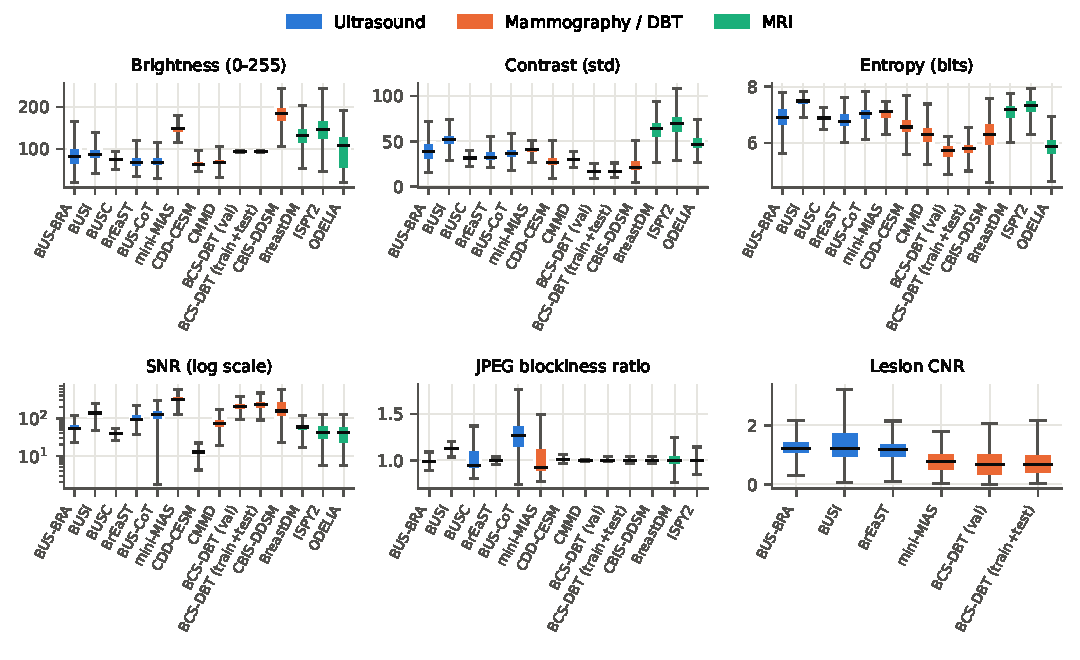
\includegraphics[width=\textwidth]{figures/quality_overview.pdf}
  \caption{Distributions of image statistics for training images, by dataset (boxes: interquartile range; whiskers: 5--95\%). Lesion CNR is shown only for datasets with masks or boxes.}
  \label{fig:quality}
\end{figure}

Table~\ref{tab:quality} and Figure~\ref{fig:quality} show large differences
between datasets even within one modality:
\begin{itemize}
  \item \textbf{Native bit depth.} The CMMD DICOMs store only 8 bits, so
  converting them to 8-bit PNG loses nothing. BCS-DBT stores 10 bits, so the
  current 8-bit crops do lose precision.
  \item \textbf{Brightness and contrast.} The digitized films of mini-MIAS are
  much brighter than the digital mammograms, and the tomosynthesis slices have
  the lowest contrast.
  \item \textbf{JPEG history.} \busiBlocky\% of BUSI images have a blockiness
  ratio above 1.05, even though they are distributed as PNG: they were
  JPEG-compressed before release.
  \item \textbf{Size heterogeneity.} BUS-BRA has 713 distinct image sizes and
  BUSI 639; CMMD and mini-MIAS each have a single size.
\end{itemize}

\subsection{Duplicates and split leakage}

\begin{table}[!htbp]
  \centering
  \small
  \caption{Integrity checks. Duplicate groups are SSIM-confirmed; leak pairs are duplicates in different training splits or folds without a shared patient/case ID. Markers = calipers or measurement lines; labels = burnt-in labels outside the breast (mammography).}
  \label{tab:integrity}
  \resizebox{\textwidth}{!}{%
  \begin{tabular}{@{}l r r r r r r r r@{}}
    \toprule
    Dataset & Dup.\ groups & Images & Label conflicts & Leak pairs & Markers & Text & Labels & Outlier queue \\
    \midrule
    \tableinput{generated/table_integrity.tex}
    \bottomrule
  \end{tabular}}
  \par\smallskip\footnotesize
  $^{\dagger}$AMBL: the thumbnail detector grouped 142 whole-breast lesion slices, but every candidate pair has a full-resolution SSIM of 0.47--0.62, so none is a duplicate.
\end{table}

\begin{figure}[!htbp]
  \centering
  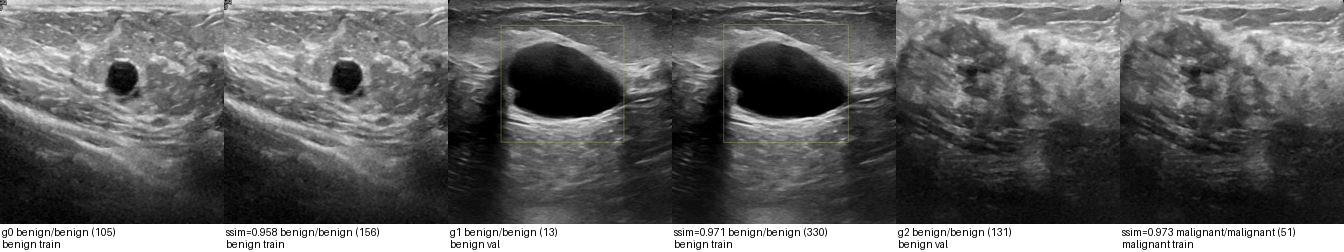
\includegraphics[width=\textwidth]{figures/busi_duplicates.png}\\[2pt]
  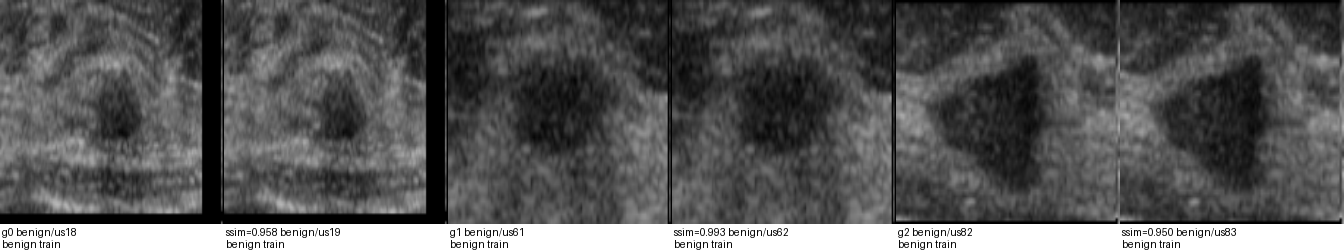
\includegraphics[width=\textwidth]{figures/busc_duplicates.png}\\[2pt]
  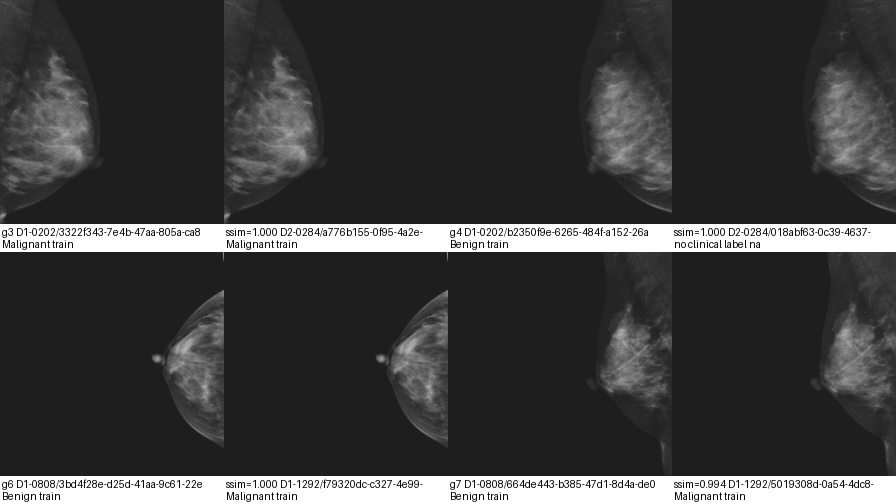
\includegraphics[width=0.67\textwidth]{figures/cmmd_duplicates.png}
  \caption{Examples of SSIM-confirmed duplicate pairs; captions give the file, label and training split. Top: BUSI, including \texttt{benign (131)} and \texttt{malignant (51)}, the same image with opposite labels, one in the validation split and one in training. Middle: BUSC consecutive frames. Bottom: CMMD images that appear under two different patient IDs.}
  \label{fig:dups}
\end{figure}

Table~\ref{tab:integrity} and Figure~\ref{fig:dups} summarize the duplicate
search. No duplicates were found \emph{between} datasets of the same modality.
Within datasets, three problems affect evaluation:
\begin{itemize}
  \item \textbf{BUSI} has 34 duplicate groups covering 75 images; 28 pairs fall
  in different training splits or folds, and 4 pairs carry opposite labels.
  BUSI has no patient identifiers, so the splitter cannot keep them together.
  \item \textbf{BUSC} has 16 groups of near-identical frames with consecutive
  file numbers, probably repeated captures of the same lesion, producing 36
  cross-split pairs.
  \item \textbf{CMMD} contains pixel-identical images (SSIM = 1.0) under
  different patient IDs: D1-0202 and D2-0284 share four images, D1-0014 and
  D1-0269 share two, and D1-0808 and D1-1292 share two with \emph{benign}
  labels for one ID and \emph{malignant} for the other. With the default seed
  every copy falls in the training split, but other seeds or folds would split them.
\end{itemize}
BUS-BRA, BrEaST, mini-MIAS, CDD-CESM and the MRI sets have no duplicates
across patients.

\subsection{Burnt-in annotations}
\label{sec:artifacts}

\begin{figure}[!htbp]
  \centering
  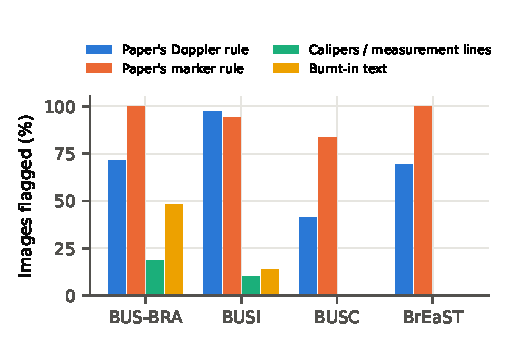
\includegraphics[width=0.55\textwidth]{figures/us_flag_rates.pdf}\\[4pt]
  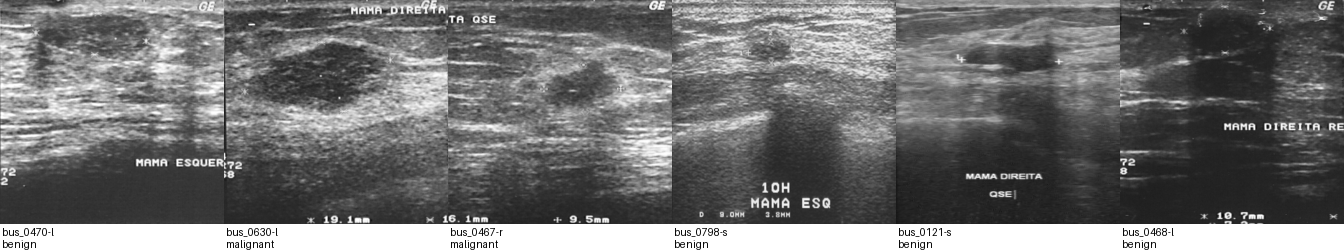
\includegraphics[width=\textwidth]{figures/busbra_text.png}
  \caption{Top: share of ultrasound images flagged by the paper's Doppler and marker rules versus our caliper and text detectors. Bottom: BUS-BRA images flagged for burnt-in text (Portuguese side labels and measurement read-outs).}
  \label{fig:flags}
\end{figure}

The paper's Doppler rule flags \busiPaperDoppler\% of BUSI images and its
marker rule \busiPaperMarker\%. On BUS-BRA the marker rule flags essentially
every image (Figure~\ref{fig:flags}), so both rules are measuring bright
tissue. Our detectors were checked by eye on random samples of their
detections: all 24 sampled caliper detections and all 24 sampled text
detections were correct. How many annotations they miss has not yet been
measured. Burnt-in annotations are common:
\begin{itemize}
  \item \textbf{BUS-BRA:} text on 898 of 1,875 images, mostly side labels and
  measurement read-outs (Figure~\ref{fig:flags}), and calipers on 349.
  \item \textbf{BUSI:} text on 108 and calipers or measurement lines on 79 of
  780 images.
  \item \textbf{BUSC and BrEaST:} none detected.
\end{itemize}
No dataset contains real colour-Doppler frames. When annotation rates differ
between classes, the annotations are a possible shortcut; the
masked-background experiments planned in the project's dataset analysis plan
will test whether models use them.

\subsection{MRI}

\paragraph{What the MRI branch receives.} In combined training, each MRI
sample is a small 2D patch cut around the tumour on one slice. The patch has
nine channels: the same location imaged at nine moments while the contrast
agent flows in and out (DCE-MRI). The shape of this time curve is the main
clinical cue for malignancy, since malignant tumours tend to enhance quickly
and wash out. Two datasets supply the patches:
\begin{itemize}
  \item \textbf{BreastDM:} 232 patients, both benign and malignant.
  \item \textbf{ISPY2:} 982 patients, all malignant (every trial participant
  has confirmed invasive cancer).
\end{itemize}

\paragraph{Patient-level statistics.} Table~\ref{tab:mri} summarizes the 3D
data behind the patches, one row per dataset:
\begin{description}
  \item[Phases] Number of contrast time points per scan. ISPY2 has a median of
  7, and some patients have only 4--6. BreastDM provides three derived
  sequences (pre-contrast, second post-contrast, subtraction) in its 3D arrays.
  \item[Volume] Tumour size. ISPY2 tumours are large (median 18\,ml), as
  expected from the trial's $\geq$2.5\,cm entry rule. BreastDM's arrays carry
  no voxel spacing, so its volume cannot be computed.
  \item[Tumour slices] Slices the tumour spans. BreastDM 6 versus ISPY2 34, so
  each ISPY2 patient contributes far more patches.
  \item[Components] Number of separate pieces the tumour mask breaks into:
  one clean region for BreastDM, a median of \ispyComponents{} fragments for ISPY2.
  \item[Enhancement ratio] Peak tumour intensity divided by pre-contrast
  intensity. The two rows are not directly comparable, because BreastDM's
  arrays were already intensity-normalized by its authors.
  \item[Lesion CNR] How strongly the tumour stands out from the surrounding
  tissue. Both datasets show clearly visible tumours (2--4).
\end{description}

\begin{table}[!htbp]
  \centering
  \small
  \caption{Patient-level MRI statistics from the 3D data: median [interquartile range]. Components = connected pieces of the tumour mask.}
  \label{tab:mri}
  \resizebox{\textwidth}{!}{%
  \begin{tabular}{@{}l r c c c c c c@{}}
    \toprule
    Source & Patients & Phases & Volume (ml) & Tumour slices & Components & Enh.\ ratio & Lesion CNR \\
    \midrule
    \tableinput{generated/table_mri.tex}
    \bottomrule
  \end{tabular}}
\end{table}

\begin{figure}[!htbp]
  \centering
  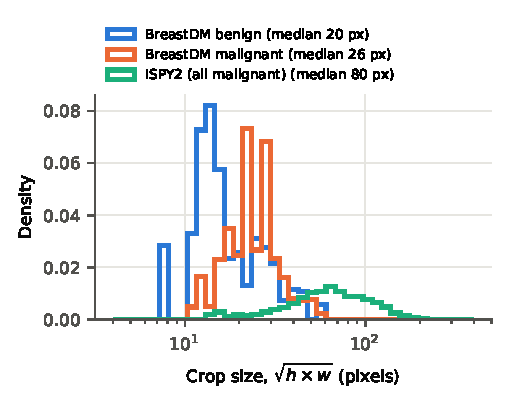
\includegraphics[width=0.5\textwidth]{figures/mri_crop_sizes.pdf}
  \caption{Size of the per-slice tumour crops fed to the MRI branch. ISPY2 crops are about three times larger than BreastDM crops of the same class.}
  \label{fig:mri}
\end{figure}

\paragraph{Finding 1: the source shortcut.}
\begin{itemize}
  \item \emph{Test.} Can a simple model tell which dataset a malignant patch
  came from without looking at the tumour itself? We trained a logistic
  regression on five numbers per patch (height, width, brightness, contrast,
  entropy) to separate ISPY2 patches from BreastDM \emph{malignant} patches.
  This is a ``name the dataset'' test~\citep{torralba2011bias}.
  \item \emph{Result.} Cross-validated AUC \probeAll{}, i.e.\ almost perfect.
  Crop size alone reaches \probeSize{}; intensity alone \probeIntensity{}.
  ISPY2 patches are about three times larger than BreastDM patches of the
  same class (Figure~\ref{fig:mri}).
  \item \emph{Why it matters.} ISPY2 contributes only malignant patches, so in
  combined training ``large patch'' almost always means ``malignant''. A model
  can score well by learning patch size instead of tumour appearance, and that
  accuracy would not transfer to data from another hospital.
  \item \emph{Cause.} Both datasets are resampled to 1\,mm voxels, so this is
  not a pixel-spacing difference. It comes from the crop rule (BreastDM: the
  smallest square around the tumour; our ISPY2 preprocessing: the mask's
  bounding box plus a 6-pixel margin) and from the trial's minimum tumour size.
  Within BreastDM, malignant patches are also larger than benign ones (median
  26 vs 20 pixels), which is partly a genuine size difference.
\end{itemize}

\paragraph{Finding 2: repeated channels.}
\begin{itemize}
  \item \emph{What happens.} The model expects nine time points, but
  \ispyRepeated{} of \ispyCases{} ISPY2 patients have fewer than nine (range
  \ispyPhasesMin--\ispyPhasesMax). The preprocessing still picks nine evenly
  spaced phase indices, so some phases are copied into two channels.
  \item \emph{Why it matters.} Channel $k$ in an ISPY2 patch does not
  correspond to the same moment as channel $k$ in a BreastDM patch, so the two
  sources present differently aligned time curves --- another difference a
  model can exploit.
\end{itemize}

\paragraph{Finding 3: fragmented masks.}
ISPY2 tumour masks are split into a median of \ispyComponents{} separate
pieces, whereas each BreastDM mask is a single region. Because the ISPY2
preprocessing makes a patch for every slice containing any mask pixels, many
ISPY2 patches show only a fragment or the edge of the tumour.

\paragraph{What to do.} Crop both sources with the same rule and a fixed
physical size; build the nine channels from matching time points
(pre-contrast, early, peak, late); and report MRI accuracy separately for
BreastDM and ISPY2, so a shortcut shows up as a gap between them.

\paragraph{Storage note.} All BreastDM \texttt{seg3D} arrays hold whole
numbers from 0 to 255, but \breadmFloatCases{} of \breadmCases{} cases are
stored as float64 (8 bytes per value instead of 1). Converting them to uint8
is lossless and makes them about eight times smaller.

\subsection{Newly added datasets}
\label{sec:new}

\paragraph{BUS-CoT overlaps the existing ultrasound data.} The cross-dataset
duplicate search matched \buscotOverlap{} BUS-CoT images to images already used
here: every one of its 1,875 BUS-BRA and 780 BUSI images
(Table~\ref{tab:buscot}). Combining BUS-CoT with BUSI or BUS-BRA would put
identical images in training and test. In \buscotRelabelled{} of these
matches BUS-CoT gives a different label than BUSI, several of them the same
BUSI images flagged earlier for conflicting duplicate labels, which makes
BUS-CoT a useful second opinion on them. The genuinely new clinical images
(TFUSL, Thammasat, UDIAT, BI-RADS ultrasound) total \buscotUsable{} images of
\buscotUsablePatients{} patients, but 36\% of the Thammasat images are
near-duplicates of each other, so it needs de-duplication first.

\begin{table}[!htbp]
  \centering
  \small
  \caption{BUS-CoT by source. ``Already used'' = images matching an image in BUSI or BUS-BRA; ``in duplicate groups'' = within BUS-CoT; ``new'' = clinical source not already in the project.}
  \label{tab:buscot}
  \begin{tabular}{@{}l r r r r r c@{}}
    \toprule
    Source & Images & Benign & Malignant & Already used & In duplicate groups & New \\
    \midrule
    \tableinput{generated/table_bus_cot.tex}
    \bottomrule
  \end{tabular}
\end{table}

\paragraph{ODELIA has a centre shortcut.} The six centres contribute very
different shares of benign lesions, from 10\% in Nijmegen to 70\% in Aachen
(Table~\ref{tab:odelia}), and their protocols differ enough that a logistic
regression on eight whole-breast statistics identifies the centre with
\odeliaCentreAcc\% accuracy (chance \odeliaCentreChance\%). The centre alone
predicts benign versus malignant with AUC \odeliaCentreOnlyAUC{}, and the same
image statistics reach only \odeliaStatsAUC{}, so most of that signal is the
centre. A model can therefore learn ``looks like Aachen $\Rightarrow$
benign''. The number of post-contrast phases also differs by centre (2 in
Cambridge, 4--5 elsewhere), so fixed multi-phase channel stacks would repeat
phases, as in ISPY2. No duplicates and no unreadable files were found.

\begin{table}[!htbp]
  \centering
  \small
  \caption{ODELIA breasts by centre. $^{*}$Held out as the out-of-distribution test centre in the ODELIA challenge.}
  \label{tab:odelia}
  \begin{tabular}{@{}l r r r r r@{}}
    \toprule
    Centre & No lesion & Benign & Malignant & Benign share of lesions & Post-contrast phases \\
    \midrule
    \tableinput{generated/table_odelia.tex}
    \bottomrule
  \end{tabular}
\end{table}

\paragraph{CBIS-DDSM's official split mixes patients.} \cbisCrossSplitPatients{}
patients (\cbisCrossSplitCrops{} crops) have a mass in one official split and a
calcification in the other, because the mass and calcification subsets were
split separately. No duplicates were found within CBIS-DDSM or between any of
the six mammography and tomosynthesis sets (\mgCrossCandidates{} candidate pairs
checked). Burnt-in film labels appear outside the breast on \cbisFullLabels{} of
\cbisFull{} full mammograms; the tight lesion crops never show them.

\paragraph{BCS-DBT training and test releases} add 321 biopsied views without
duplicates or patient overlap with the validation release, from the same
single vendor (Hologic Selenia Dimensions).

\subsection{Datasets added 19--22 October}
\label{sec:new2}

Three more datasets were downloaded and audited with the same pipeline:
AMBL (MRI, the 99 patients with lesion masks), DMID (mammography) and BUS-UCLM
(ultrasound). Their rows appear in Tables~\ref{tab:counts}--\ref{tab:integrity}.
BUS-UCLM and DMID share no images with the other datasets of their modality
(\mgCrossCandidates{} mammography candidate pairs checked); the MRI sets are not
cross-checked.

\paragraph{AMBL: the masks do not say which lesion is benign.} Every DICOM
SEG segment is labelled only ``Mass''. The clinical sheet lists each lesion's
side and benign/malignant outcome, and its data dictionary says the segments
list all tumours first, then all benign lesions. Checking each mask's side
against the sheet, that ordering puts 20\% of the masks in the wrong breast
(tumour and benign swapped, e.g.\ AMBL-008 and AMBL-011). Labels were
therefore resolved per patient:
\begin{itemize}
  \item one label for all of a patient's lesions: 109 lesions;
  \item otherwise by the mask's side, where each breast holds one label: 29;
  \item otherwise excluded as ambiguous: 27.
\end{itemize}
This leaves 138 lesions (68 benign, 70 malignant) in 92 patients. The
resolved labels behave like real malignancy. Malignant lesions enhance faster
(initial enhancement alone gives AUC 0.77), and most benign lesions keep
enhancing to the last phase (46 of 68, against 23 of 70 malignant). Lesion
size separates the classes even more strongly (AUC 0.83; median 2.8 vs.\
0.37\,ml), and it stays the strongest single predictor: on these lesions a
ResNet-18 reached a lesion-level AUC of 0.72 against 0.85 for size alone.
Further points:
\begin{itemize}
  \item Six patients (7 lesions) are post-chemotherapy scans and should be
  excluded from a diagnosis benchmark.
  \item The masks are fragmented: median 15 connected pieces for malignant
  lesions, from the thresholded annotation.
  \item The segmentations reference the registered DCE series, which shares
  the original series' slice grid, so the masks place correctly on the
  original images.
  \item The label counts differ from the BreastDCEDL\_AMBL benchmark (133
  lesions, 89 benign / 44 malignant), so that paper's patient selection or
  label mapping is not the one in the TCIA clinical file.
\end{itemize}

\paragraph{DMID: side predicts the label, and there are no patient IDs.}
\begin{itemize}
  \item \textbf{Laterality.} 62\% of malignant images are left breasts
  against 40\% of benign ($p=0.0003$), so laterality alone gives AUC 0.61.
  Breast orientation reveals the side, so a CNN can learn this shortcut.
  \item \textbf{No patient identifier.} Every image is its own study and
  no patient field exists, so a patient's CC and MLO views cannot be kept on
  one side of a split.
  \item \textbf{Three duplicate pairs} (SSIM $\geq$ 0.999). One pair is
  labelled undefined in one copy and benign in the other.
  \item \textbf{Labels and masks.} 20 images contain both a benign and a
  malignant finding. 268 of the 276 benign or malignant images have a usable
  ROI mask: 7 have none and 1 file is corrupt.
  \item \textbf{Burnt-in film labels} appear on 68--82\% of images, more often
  on normal ones. This could be a shortcut for normal vs.\ abnormal.
  \item \textbf{Lesion size} alone gives AUC 0.70.
\end{itemize}

\paragraph{BUS-UCLM: one patient under two IDs.} Four images of patient
``CHCO'' are pixel-identical to images of ``CHVI'', so the two prefixes are
one patient and must be merged before any patient-level split. The other
duplicate pairs are consecutive frames of the same patient. Mask colours agree
with the labels on every image. Caliper marks appear on 52\% of benign and
60\% of malignant images but carry little label information (AUC 0.54), and
Doppler is weaker still (AUC 0.56). Our caliper detector does not recognise
this scanner's markers, so the dataset's own flags are used instead. Lesion
size gives AUC 0.66. Five of 38 patients have both benign and malignant
images.

\subsection{Findings from preparing the data for training}
\label{sec:prep}

Preparing the new datasets for training (16--19 October 2026) surfaced
further properties of the data. None of them changes the counts above.

\paragraph{ODELIA's subtraction volumes are padded with a negative constant.}
Outside the breast, \texttt{Sub\_1} is filled with a large negative value that
differs by centre (for example $-891$ in Cambridge, $-821$ in Aachen and
$-1{,}997$ in Utrecht), and the pre-contrast and T2 volumes start at 0. A
percentile intensity window over the whole volume therefore maps tissue with
no enhancement to mid-grey, differently per centre. The MRI-branch conversion
windows \texttt{Sub\_1} to $[0,\,\text{99.5th percentile of positive voxels}]$
instead. Picking the axial slice with the most enhancement, as a mask-free
lesion locator, mostly selected the heart and chest wall at the image edge,
so the central slice is used. The cached volumes are faithful to the release:
the authors' published classifier, scored on our cache, reproduces their
reported macro AUC exactly (81.6 in distribution, 63.1 on the Valencia centre).

\paragraph{BUS-CoT's classification set and its new clinical part.} The
\texttt{BUS-Lesion} set the paper benchmarks holds 5,163 lesion images (2,694
benign, 2,469 malignant) with an official patient-level split of 4,338
\emph{trainval} and 825 \emph{test} images; no patient appears in both.
Restricted to the new clinical sources and de-duplicated with the audit's
duplicate groups (one image kept per group, groups with conflicting labels
dropped), it leaves 2,036 images: TFUSL 1,575, Thammasat 349 and UDIAT 112.
STU-Hospital and the BI-RADS ultrasound set do not appear in \texttt{BUS-Lesion}.

\paragraph{ISPY2 response labels.} The BreastDCEDL metadata file supplies the
pathologic complete response (pCR) label for all 982 ISPY2 patients (32\%
pCR) and the authors' fixed split, which for ISPY2 is 784 / 99 / 99
patients. Its split column is coded 0/1/2; across all three cohorts, codes 1
and 2 hold 177 and 176 patients at 29.9\% and 30.1\% pCR, which identifies
them as the paper's validation and test sets. These labels describe treatment
response, not benign versus malignant, so ISPY2 stays malignant-only in the
fusion model.

\paragraph{Patient-level splits for CBIS-DDSM and BCS-DBT.} All 2,006 CBIS-DDSM
crops converted without loss of any sample. Shen's 85/15 patient split with a
10\% validation hold-out gives 823 / 91 / 161 patients with none shared. The
three BCS-DBT releases together give 396 biopsied views from 201 patients. The
BCS-DBT detection baseline cannot be checked on this data: its authors never
released trained weights.

\paragraph{Ultrasound preprocessing changes more than intended.} Two classical
steps from the project's earlier preprocessing work were measured on BUS-BRA
and BrEaST samples. Morphological line removal (top-hat and black-hat
responses thresholded with Otsu's method, then inpainted) altered 15--91\% of
the pixels at both of its tested settings, because speckle passes the
threshold as ``lines''. The narrower caliper-cross removal altered 2--22\%.
The earlier intensity-normalization step mapped 0--255 to 0--255 with
clipping, which leaves 8-bit images unchanged.

\begin{figure}[!htbp]
  \centering
  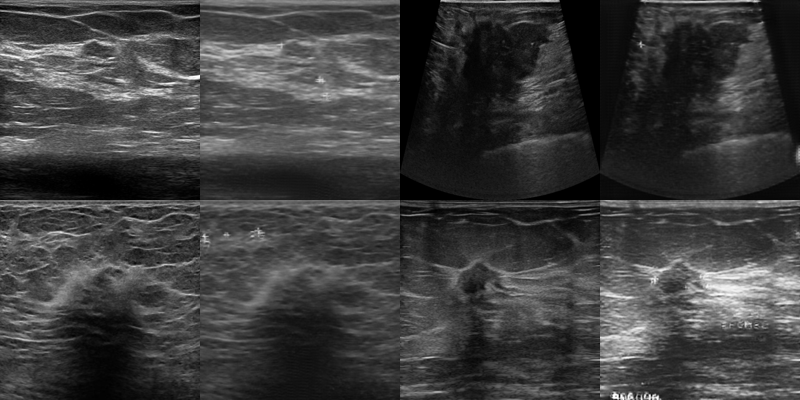
\includegraphics[width=\textwidth]{figures/cyclegan_calipers.png}
  \caption{Four BrEaST images (left of each pair) and their CycleGAN translation towards BUS-BRA's appearance (right). The translations gain caliper crosses on the lesions and measurement text near the bottom edge, which are absent from the BrEaST originals.}
  \label{fig:cyclegan}
\end{figure}

\paragraph{A style-transfer model learns the burnt-in annotations.} A CycleGAN
trained to translate BrEaST images into BUS-BRA's appearance adds caliper
crosses and measurement text to the translated BrEaST images, placed on or
next to the lesion (Figure~\ref{fig:cyclegan}). BrEaST has no burnt-in annotations
(Section~\ref{sec:artifacts}), so the generator learned BUS-BRA's annotations
as part of its ``style''. This is direct evidence that the BUS-BRA annotations
are a consistent, learnable image property. A classifier could use them the
same way, which strengthens the case for the annotation-shortcut experiments
below.

\section{Recommendations}
\label{sec:recommendations}

\begin{enumerate}
  \item \textbf{Group duplicates before splitting.} Treat each duplicate group
  as a single ``patient'' in BUSI and BUSC, merge the duplicated CMMD patient
  IDs, and drop or adjudicate the five benign/malignant conflicts (4 BUSI,
  1 CMMD patient pair). Re-run the BUSI and BUSC baselines afterwards.
  \item \textbf{Report pathology confirmation alongside results.} Results on
  BUSI, BUSC and mini-MIAS rest on radiologist labels, and BrEaST and CDD-CESM
  partly on follow-up. These are weaker references than the biopsy- or
  histology-confirmed BUS-BRA, CMMD, BCS-DBT, BreastDM and ISPY2 labels.
  \item \textbf{Remove the MRI source shortcut.} Use the same crop geometry
  and intensity normalization for ISPY2 and BreastDM, build the nine channels
  from matching time points, and report MRI metrics separately for each source.
  \item \textbf{Test annotation shortcuts} in BUS-BRA and BUSI with
  masked-background and inpainted-annotation experiments.
  \item \textbf{Keep 16-bit data where it exists.} Re-prepare BCS-DBT crops as
  16-bit PNG; for CMMD, 8-bit PNG is already lossless.
  \item \textbf{Use only the new part of BUS-CoT.} Exclude its BUSI and
  BUS-BRA copies and the scraped web and figure sources; de-duplicate the
  Thammasat images before splitting.
  \item \textbf{Evaluate ODELIA leave-one-centre-out} (at minimum keep
  Valencia unseen), report results per centre, compare against the
  centre-only baseline (AUC \odeliaCentreOnlyAUC), and use the pre-contrast,
  subtraction and T2 volumes that every centre has.
  \item \textbf{Split CBIS-DDSM by patient} when mass and calcification crops
  are used together, and report results with and without the
  BENIGN\_WITHOUT\_CALLBACK crops.
  \item \textbf{Avoid morphological line removal on B-mode images}; use the
  caliper-cross removal or a learned marker remover, and inspect a preview
  before training on any preprocessed set.
  \item \textbf{Remove annotations before training a style-transfer model} on
  BUS-BRA (or any annotated source), otherwise the translated images inherit
  calipers and text placed on the lesion.
  \item \textbf{AMBL:} use the side-checked labels, exclude ambiguous lesions
  and post-chemotherapy scans, and report lesion size as the baseline any
  model must beat.
  \item \textbf{DMID:} report a laterality-only baseline (or flip all images to
  one side), keep one image per duplicate pair, and state that splits are
  image-level.
  \item \textbf{BUS-UCLM:} merge the CHCO and CHVI prefixes before splitting by
  patient.
\end{enumerate}

\paragraph{Status (19 October 2026).} Recommendations 6--8 are in place in
training: only BUS-CoT's de-duplicated clinical part enters the fusion
model; ODELIA is trained and tested per fold with Valencia held out and
uses pre-contrast, subtraction and T2; CBIS-DDSM is split by patient, with
BENIGN\_WITHOUT\_CALLBACK excluded by default. In the fusion model, MRI is
now reported per source, so ISPY2 no longer hides inside a pooled MRI
score. Recommendations 1--5 and 9--10 are still open.

\section{Planned datasets not yet analysed}
\label{sec:planned}

The project's intake plan lists further datasets that are not downloaded or
not yet audited (Table~\ref{tab:planned}). None of the numbers in this report
cover them.

\begin{table}[!htbp]
  \centering
  \footnotesize
  \caption{Planned datasets not yet analysed (status 22 October 2026).}
  \label{tab:planned}
  \begin{tabularx}{\textwidth}{@{}l l Y Y@{}}
    \toprule
    Dataset & Mod. & Access & Status / reason not analysed \\
    \midrule
    VinDr-Mammo & MG & PhysioNet, restricted: account + data-use agreement & Access request to be submitted; 5,000 four-view exams, BI-RADS labels with pathology for a subset only \\
    CSAW-CC & MG & Karolinska / Swedish National Data Service, by request & Access request to be submitted; 873 cancers and 7,850 controls, Hologic only \\
    AMBL, remaining patients & MRI & TCIA / IDC, open & 101 further patients with clinical labels but no lesion masks (about 36\,GB); not downloaded \\
    I-SPY1 (+ Tumor-SEG) & MRI & TCIA, open (Data Retriever) & Not downloaded; malignant-only, like ISPY2 \\
    I-SPY2 full collection & MRI & TCIA, open (about 1.75\,TB) & Only the BreastDCEDL subset is held; the full collection exceeds local storage \\
    Breast-MRI-NACT-Pilot & MRI & TCIA, open (about 19.5\,GB) & Not downloaded; 64 patients, treatment response \\
    Mammo-MX & MG & Open (about 75\,GB) & Deferred for storage \\
    UDIAT Dataset B & US & Author page, by request & Not requested; BUS-CoT already includes part of it \\
    BUSIS & US & Author-distributed & Not requested \\
    BUID (QAMEBI) & US & Open, separate benign/malignant archives & Not downloaded \\
    Breast ultrasound videos; ``eight-diagnosis'' database & US & -- & Not identified: no public release matches these names \\
    \bottomrule
  \end{tabularx}
\end{table}

\section{Limitations}

\begin{itemize}
  \item \textbf{Approximate image metrics.} Thumbnail SSIM can miss duplicates
  that were heavily re-cropped, so embedding-based duplicate search is planned.
  \item \textbf{Unmeasured detector misses.} The artifact detectors were
  checked for false detections but not for missed annotations.
  \item \textbf{Citation counts change.} They come from one source on one date.
  \item \textbf{BUS-CoT sources are identified indirectly.} The paper does not
  name TFUSL and TUHD; their identification is our best match.
  \item \textbf{ODELIA statistics use a projection.} Its image statistics are
  computed on the subtraction maximum-intensity projection of each breast, so
  they are not directly comparable with the other datasets' per-image values.
  \item \textbf{Prepared-data analyses not yet run.} Texture features,
  embedding-based dataset shift, label-noise detection and shortcut ablations
  are still to come.
\end{itemize}

\bibliographystyle{plainnat}
\bibliography{references}

\end{document}
